As I understand the question, we should assume that the event of whether a passenger with a flight reservation shows up or not is drawn from a bernoulli distribution with a given probability $p$ of showing up, and a probability $1-p$ of not showing up. Using this assumption, we have to bound the probability that the following two events both happen: 
\begin{itemize}
\item Event $A$: We i.i.d sample 1000 flight reservations from the distribution, and the passengers show up in exactly in 95 percent of them.
\item Event $B$: We i.i.d sample 100 flight reservations from the distribution, and the passengers show up in all of them.
\end{itemize}
Since event $A$ and event $B$ are independent, then $P_p(A \land B) = P_p(A)P_p(B)$, where $p$ is the probability of a single passenger showing up for a reservation. $P_p(A)P_p(B)$ probability is going to be very low, however, since the probability of observing \textit{exactly} 95 percent of the passengers in the 10000 reservations not showing up is very low, no matter what $p$ is. To be precise, this probability is equal to the value of the binomial distribution of 9500 success in 10000 experiments with a success probability $p$ on each experiment. I denote this value by $\text{bin}(9500, 10000,p)$. In other words, we have:
\begin{align}
P_p(A) = \text{bin}(9500, 10000,p)
\end{align}
As in question 1, we also have that:
\begin{align}
P_p(B) = p^{100}
\end{align}
All in all, we therefore have that:
\begin{align}
P_p(A \land B) = P_p(A)P_p(B) = \text{bin}(9500, 10000,p) p^{100}
\end{align}
Here are two plots of the probability of the flight company getting unlucky, that is $P_p(A \land B)$, against the value of $p$. The plot on the right is just a zoomed in version of the plot on the left, only focusing on $p$ from 0.94 to 0.96:
\begin{center}
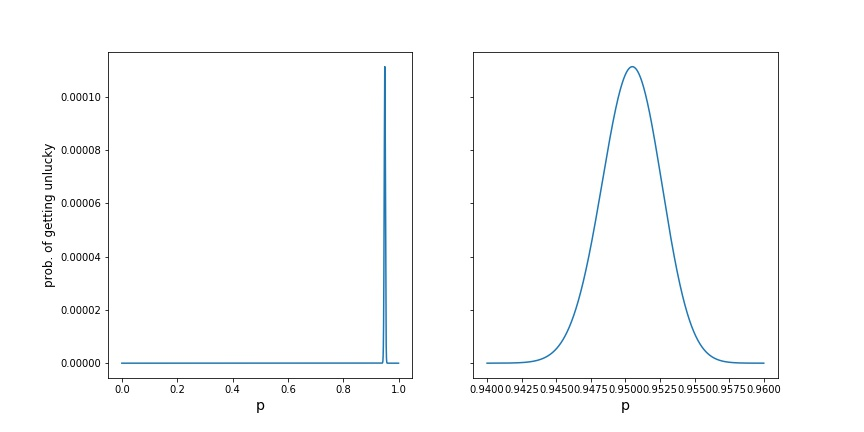
\includegraphics[scale=0.5]{airline_revisited/fig1.jpg}
\end{center}
The value of $P_p(A \land B)$ is maximized for $\tilde{p}=0.95005$ with a value of $P_{\tilde{p}}(A \land B)=0.00011$. This means that for all $p \in [0,1]$, we have that $P_p(A \land B) \leq 0.00011$. However, this says very little about anything interesting, since the low probability just comes from the fact that we are taking $A$ as the event of observing \textit{exactly} 95 percent of the passengers not showing up. A flight company would be completely uninterested in this probability, since they would never have a decision procedure of implementing the reservation policy of overbooking with 1 passenger, if and only if they observe exactly event $A$ happening. 

Another slighty more interesting, but still not very realistic scenario, is to ask for the probability of observing both event $\hat{A}$ and event $B$, where
\begin{itemize}
\item Event $\hat{A}$: We i.i.d sample 1000 flight reservations from the distribution, and the passengers show up in exactly in less than or exactly 95 percent of them.
\item Event $B$: We i.i.d sample 100 flight reservations from the distribution, and the passengers show up in all of them.
\end{itemize}
Here we have that $P_p(\hat{A})$ is just the value of the cumulative binomial distribution of 9500 success in 10000 experiments with a success probability $p$ on each experiment. I denote this value by $\text{cumbin}(9500, 10000,p)$. We therefore have:
\begin{align}
P_p(\hat{A} \land B) = P_p(\hat{A})P_p(B) = \text{cumbin}(9500, 10000,p) p^{100}
\end{align}
Here are two plots of the probability of the flight company getting unlucky in this setting against the value of $p$:
\begin{center}
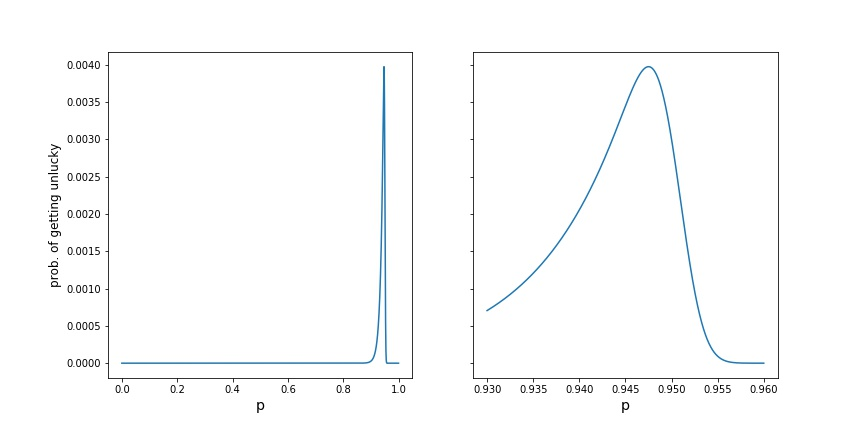
\includegraphics[scale=0.5]{airline_revisited/fig2.jpg}
\end{center}
The value of $P_p(\tilde{A} \land B)$ is maximized for $\tilde{p}=0.94475$ with a value of $P_{\tilde{p}}(\hat{A} \land B)=0.0039$. This means that for all $p \in [0,1]$, we have that $P_p(\hat{A} \land B) \leq 0.0039$.
